\chapter{Diseño e Implementación} % Main chapter title

\label{Chapter3} % Change X to a consecutive number; for referencing this chapter elsewhere, use \ref{ChapterX}

En este capítulo se explican con detalle todo los elementos que componen al sistema y los criterios utilizados para su desarrollo. Se parte de una breve descripción de la estructura del sistema, pasando por el desarrollo de los módulos de hardware y se concluye con la implementación del software.


\section{Estructura general del sistema}
Con el objetivo de lograr un sistema adaptable y escalable se optó por realizar un diseño modular. Este diseño consiste en tres tipos de módulos o etapas: el módulo principal, los módulos adicionales y la interfaz de usuario. La figura \ref{fig:BloquesGral} indica en forma general la estructura del sistema y el modo en que los módulos están conectados entre sí.


\begin{figure}[ht]
	\centering
	\includegraphics[scale=0.5]{./Figures/BloquesGral.pdf}
	\caption{Diagrama en bloques del sistema.}
	\label{fig:BloquesGral}
\end{figure}

\subsection{Módulo principal}
El módulo principal es la base del sistema, allí se encuentra el núcleo de procesamiento, la etapa de comunicación con la interfaz de usuario, el servidor web de la misma y los puertos de conexión con los módulos adicionales. Estos puertos de conexión son los encargados de capturar las señales provenientes de los módulos adicionales, tanto en forma analógica como digital. Además, son capaces de generar señales analógicas y digitales y proveer de alimentación a los módulos adicionales.
Una característica importante de estos puertos de conexión es que se encuentran aislados eléctricamente uno del otro para poder trabajar con equipos no aislados y únicamente se  comunican con el núcleo de procesamiento mediante una interfaz optoaislada.

\subsection{Módulos adicionales}
Los módulos adicionales cumplen las funciones de conectar y adaptar las señales entre los puertos del módulo principal y el equipo bajo prueba. Estos módulos se diseñan específicamente para cada tipo o familia de productos. Gracias a esta estructura modular se puede adaptar el sistema para realizar distintas pruebas con pocos cambios de hardware.
Al momento se desarrollaron dos módulos adicionales, uno para prueba de temporizadores y otro para la prueba de salida de drivers.

\subsection{Interfaz de Usuario}
La interfaz de usuario es el medio por el cual se controla al sistema. Se desarrolló de forma que pueda ejecutarse en cualquier plataforma que tenga un navegador web y esté conectada a la misma red que el módulo principal. Por ejemplo, se puede ejecutar desde una tablet, notebook o celular y con solo ingresar el IP del sistema de pruebas se tiene acceso al panel de control donde se puede seleccionar la prueba a realizar, configurar los parámetros, ejecutar las pruebas y visualizar los resultados.

\section{Desarrollo de hardware del módulo principal}

El módulo principal, como se mencionó anteriormente, posee el núcleo de procesamiento implementado con una placa de desarrollo EDU-CIAA, un módulo de comunicación WIFI ESP-01 para la interfaz de usuario y los puertos de conexión con los módulos adicionales. En la figura \ref{fig:BloquesPrincipal} se presenta un diagrama en bloques del módulo principal cuyos elementos serán detallados a continuación.

\begin{figure}[H]
	\centering
	\includegraphics[width=1\textwidth]{./Figures/bloquesPrincipal.pdf}
	\caption{Diagrama en bloques del módulo principal.}
	\label{fig:BloquesPrincipal}
\end{figure}



\subsection{Placa de desarrollo EDU-CIAA}

El uso de la placa de desarrollo EDU-CIAA como núcleo de procesamiento fue uno de los requerimientos establecidos al inicio del proyecto. Esta decisión se basó principalmente en que la EDU-CAA es la plataforma sobre la que más se trabajó durante la especialización y se dispone de gran variedad de recursos de software y soporte por parte de la comunidad. 
Respecto al hardware, la placa dispone un procesador LPC4337 con dos núcleos asimétricos, un Cortex M4 y un Cortex M0, trabajando a 208 Mhz y un amplio abanico de interfaces de comunicación como ser bus I2C, SPI, USB, CAN y varias UARTs. 


\subsection{Puertos de conexión}

Los puertos de conexión son las piezas de hardware que más trabajo requirieron en su diseño. Fue necesario desarrollar dos esquemas preliminares de hardware a causa de que las primeras pruebas que se realizaron no fueron exitosas. Esto se debió a que el diseño no contemplaba el hecho de que muchos drivers de LEDs no están aislados entre entrada y salida, impidiendo así el uso de una masa común entre los distintos puertos de conexión. Siendo imposible solucionar esto sin alterar la topología del circuito, se optó por un esquema de puertos opto-aislados. La figura \ref{fig:BloquesPuerto} representa en un esquema de bloques el circuito de un puerto de conexión donde se puede apreciar que cada puerto dispone de un microcontrolador de la familia STM32, en particular para el desarrollo se eligió un módulo Bluepill basado en el microcontrolador STM32F108C8T6 con núcleo Cortex M3. Este microcontrolador cumple las siguientes funciones:

\begin{itemize}
	\item Comunicación mediante UART opto-aislada con la EDU-CIAA.
	\item Capturar el estado de las 3 entradas digitales del puerto.
	\item Muestreo de las 2 entradas analógicas del puerto.
	\item Comunicación con el conversor digital-analógico de la salida analógica 0-10v.
	\item Generar las señales de las 3 salidas digitales del puerto y activar el relay de alimentación de 220VAC.
\end{itemize}

\begin{figure}[ht]
	\centering
	\includegraphics[width=1\textwidth]{./Figures/BloquesPuerto.pdf}
	\caption{Diagrama en bloques de un puerto de conexión.}
	\label{fig:BloquesPuerto}
\end{figure}


\subsection{Interfaz UART opto-aislada}
	
Para el diseño de la interfaz UART opto-aislada se tuvieron en cuenta los requerimientos de cantidad de canales analógico a digital y digital a analógico, la velocidad de muestreo y el número de entradas y salidas digitales, que en forma indirecta establecen la velocidad de comunicación mínima que debe poseer la interfaz UART opto-aislada entre los puertos y la EDU-CIAA.
También fue necesario establecer un protocolo para empaquetar los datos e identificar a qué puerto corresponde cada paquete de datos.
El protocolo diseñado consiste en un protocolo maestro-esclavos donde un maestro, en este caso la EDU-CIAA, inicia la comunicación con un esclavo enviando una trama de 5 bytes, como lo indica la figura \ref{fig:TramaMS}, que a través de la UART opto-aislada llega a todos los puertos.

\begin{figure}[H]
	\centering
	\includegraphics[width=1\textwidth]{./Figures/TramaMS.pdf}
	\caption{Estructura de una trama de datos de maestro a esclavo.}
	\label{fig:TramaMS}
\end{figure}

A continuación cada esclavo, es decir cada uno de los puertos, captura la trama y obtiene la dirección correspondiente a la trama recibida y la compara con la propia. Solo el esclavo con la misma dirección debe responder al maestro mediante una trama de 4 bytes con la estructura que se indica en la figura \ref{fig:TramaSM}.

\begin{figure}[H]
	\centering
	\includegraphics[width=1\textwidth]{./Figures/TramaSM.pdf}
	\caption{Estructura de una trama de datos de esclavo a maestro.}
	\label{fig:TramaSM}
\end{figure}

Una vez establecido el protocolo donde se deben transmitir 5 bytes de maestro a esclavo y 4 bytes de esclavo a maestro en configuración full-duplex, y teniendo en cuenta que en el listado de requerimientos se establecio una taza de refresco de mil veces por segundo por cada uno de los seis puertos, se calculó una velocidad de comunicación mínima requerida de 30 KB/s. Luego se escogió la velocidad estándar más cercana para un puerto UART, siendo ésta 460800 Kb/s excede ampliamente lo minimo requerido y deja espacio para futuras expansiones.

Para la selección de los opto acopladores, se evaluaron algunas alternativas disponibles en el mercado local. La tabla \ref{tab:Optos} resume las características principales de los mismos donde se puede destacar al tiempo de respuesta como el factor limitante. 
Utilizando como criterio de diseño que el tiempo de respuesta del optoacoplador debe ser 10 veces menor que el tiempo de un bit para lograr una salida aceptable, significa que para lograr una velocidad de 460800 Kb/s se requiere un tiempo de respuesta menor a 217 ns. Por lo tanto en la tabla \ref{tab:Optos} se puede observar que la mejor opción para la aplicación es el optoacoplador 6N137 debido a que es el único capaz de trabajar a la velocidad de 460800 Kb/s requerida.

	\begin{table}[h]
	\centering
	\caption[Tabla de comparación de optoacopladores para la interfaz UART optoaislada]{Comparación de optoacopladores}
	\begin{tabular}{l c c c c}    
		\toprule
		\textbf{Modelo} 	 & \textbf{PC817(1)} & \textbf{4N35(2)}& \textbf{6N137(3)}	\\
		\midrule
Tensión de alimentación             & \textless{}80 V & \textless{}70 V & 5 V           &  \\
Tipo de salida                      & Transistor      & Transistor      & \emph{Open drain}    &  \\
Tiempo de respuesta subida / bajada & 18 us / 18 us   & 10 us / 10 us   & 75 ns / 75 ns &  \\
Tensión de aislación                & 5 KV            & 5 KV            & 5.3 KV        &  \\
Cantidad de pines                   & 4               & 6               & 8             & \\
		\bottomrule
		\hline
	\end{tabular}
	\label{tab:Optos}
\end{table}

Una vez seleccionado el optoacoplador se realizó el diagrama esquemático de la interfaz opto-aislada de la figura \ref{fig:InterfazOpto}. El diseño contempla que la salida, es decir la línea de datos del puerto hacia la EDU-CIAA, sea por colector y resistencia pull-up para que se puedan conectar todos los puertos en paralelo. A su vez se tuvo en cuenta que la entrada de todos los puertos están conectadas a la misma salida de la EDU-CIAA y ésta no debe ser sobrecargada, por lo que se utilizó un transistor a la entrada que actúe de buffer.

\begin{figure}[H]
	\centering
	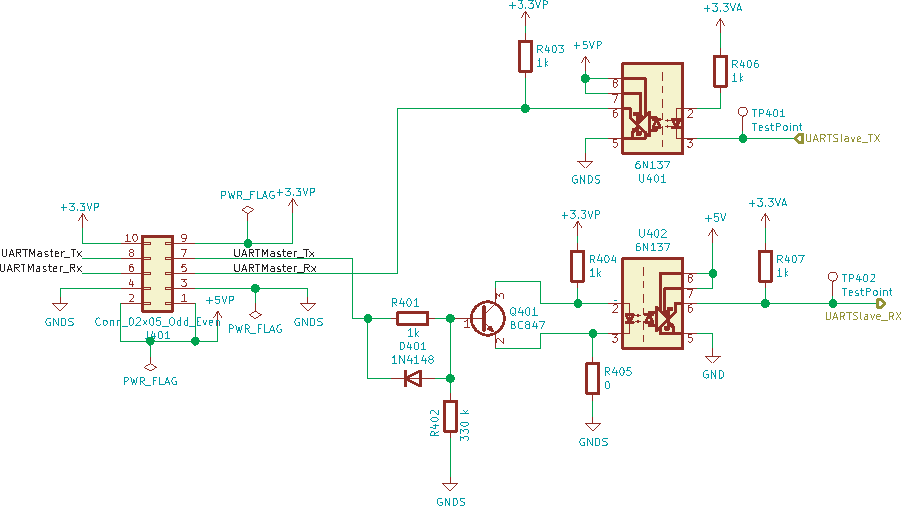
\includegraphics[width=1\textwidth]{./Figures/InterfazOpto.pdf}
	\caption{Diagrama esquematico de la interfaz UART optoaislada.}
	\label{fig:InterfazOpto}
\end{figure}


\subsection{Entradas y salidas digitales}

Del listado de requerimientos surge la necesidad de implementar tres entradas digitales, tres salidas digitales y una salida de alimentación para los módulos adicionales. La figura \ref{fig:EntradaDigital} muestra el diagrama esquemático del circuito adaptador de nivel de una de las entradas digitales la cual fue diseñada para tolerar niveles de tensión de hasta 30 V y proteger al microcontrolador STM32F108C8T6.

\begin{figure}[H]
	\centering
	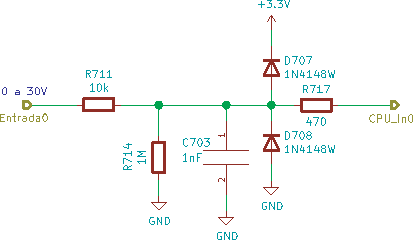
\includegraphics[width=0.8\textwidth]{./Figures/EntradaDigital.pdf}
	\caption{Diagrama esquematico de una entrada digital.}
	\label{fig:EntradaDigital}
\end{figure}

Para las salidas digitales se escogió una configuración de salida optoacoplada de colector abierto como se ve en la figura \ref{fig:SalidaDigital}. En esta misma figura, además, se puede ver la salida de alimentación de 220 VAC de los módulos adicionales, esta se implementó con una salida a relé de dos contactos que permite la conexión y desconexión de fase y neutro al mismo tiempo.

\begin{figure}[H]
	\centering
	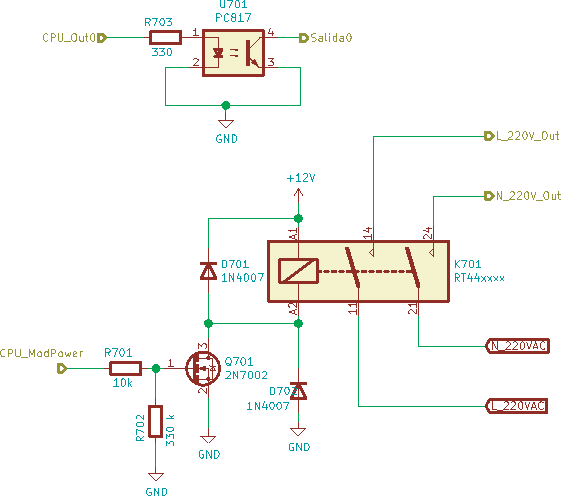
\includegraphics[width=0.8\textwidth]{./Figures/SalidaDigital.pdf}
	\caption{Diagrama esquemático de una salida digital y la salida de alimentacion de 220 VAC.}
	\label{fig:SalidaDigital}
\end{figure}

\subsection{Salida y entradas analogicas}

Cada puerto del módulo principal dispone de una salida analógica con capacidad de generar señales entre 0-10 V. Como el microcontrolador STM32F108C8T6 no posee un conversor digital analógico fue necesario utilizar un conversor externo, el conversor elegido para el diseño fue el MCP4725 de microchip. Este conversor de 12 bits y un canal se comunica con el microcontrolador mediante un bus I2C. 
Como se puede ver en el diagrama esquemático de la figura \ref{fig:SalidaAnalogica} se tuvo que diseñar una etapa de amplificación que lleve el nivel de tensión del rango 0 - 3.3 V que puede entregar el MCP4725 hasta el rango de 0 - 10 V que fue especificado en los requerimientos para la salida analógica..

\begin{figure}[H]
	\centering
	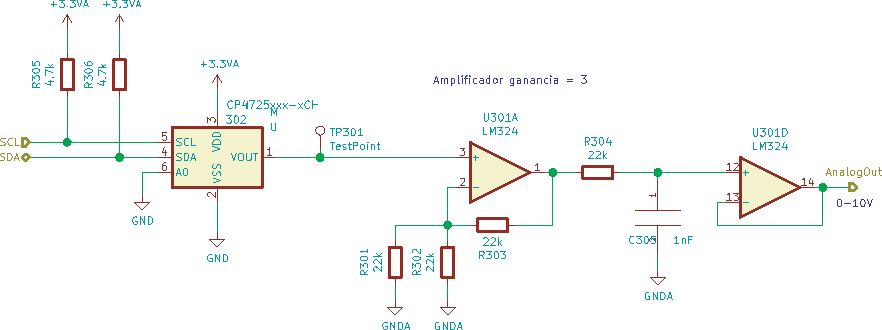
\includegraphics[width=1\textwidth]{./Figures/SalidaAnalogica.pdf}
	\caption{Diagrama esquemático de la salida analógica de un puerto.}
	\label{fig:SalidaAnalogica}
\end{figure}

Para las entradas analógicas se dio uso a los dos conversores analógico-digital incluidos en el microcontrolador STM32F103C8T6, que muestrean ambas entradas en forma simultanea. Al igual que la salida analogica, fue necesario hacer una adaptación del nivel de tensión de entrada de 0 -10 V al rango 0 - 3.3 V con un circuito atenuador y un buffer. En la figura \ref{fig:EntradaAnalogica} se puede ver el circuito atenuador implementado que además, para proteger al puerto, se diseño una protección por sobre tensión en la entrada analogica que limita la tensión a un máximo de 12 V.

\begin{figure}[H]
	\centering
	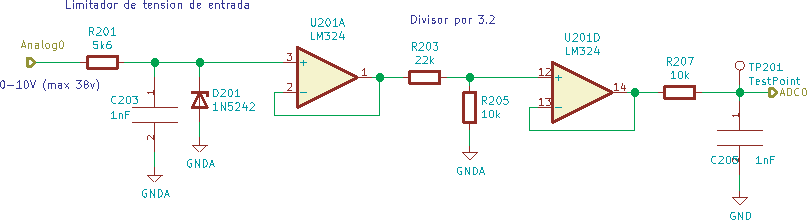
\includegraphics[width=1\textwidth]{./Figures/EntradaAnalogica.pdf}
	\caption{Diagrama esquemático de una entrada analógica.}
	\label{fig:EntradaAnalogica}
\end{figure}




\section{Desarrollo de hardware del módulo prueba de drivers}

El módulo test de drivers es un circuito diseñado para realizar la medición de los valores de tensión y corriente en la salida de un driver para iluminación LED. En el diagrama en bloques de la figura \ref{fig:BloquesTestDriver} se puede ver que el módulo está compuesto por cinco etapas que adaptan las señales a los niveles de tensión soportados por los puertos del módulo principal y la forma en que se conecta con el modulo principal y la carga.

\begin{figure}[H]
	\centering
	\includegraphics[width=1\textwidth]{./Figures/BloquesTestDriver.pdf}
	\caption{Diagrama en bloques del modulo prueba de drivers.}
	\label{fig:BloquesTestDriver}
\end{figure}


De las cinco etapas de este módulo, dos sirven para mediciones analogicas. La primera etapa, cuyo esquemático se puede ver en la figura \ref{fig:MedicionCorriente}, es para la medición de corriente de salida de drivers de LEDs. Esta se diseñó para hacer mediciones entre 0 y 2,5 A de corriente continua entregando a la salida un nivel de tensión proporcional en el rango 0 - 10 V.

\begin{figure}[H]
	\centering
	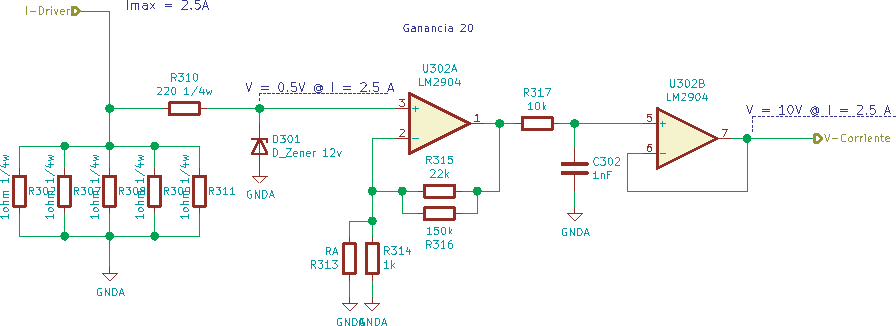
\includegraphics[width=1\textwidth]{./Figures/MedicionCorriente.pdf}
	\caption{Esquematico del circuito de medición de corriente de drivers.}
	\label{fig:MedicionCorriente}
\end{figure}

La segunda etapa de medicion analogica es una etapa de medicion de tension continua de la salida del driver de LEDs. En el esquemático de la figura \ref{fig:MedicionTension} se puede ver el circuito atenuador y separador diseñado para llevar el nivel de tensión del rango 0 - 500 VDC a 0 - 10 V compatible con los puertos del módulo principal.

\begin{figure}[H]
	\centering
	\includegraphics[width=0.7\textwidth]{./Figures/MedicionTension.pdf}
	\caption{Esquematico del circuito de medición de tensión de drivers.}
	\label{fig:MedicionTension}
\end{figure}

Este módulo además posee dos salidas para dimerizar drivers, una de ellas de dimerizado analogico, para la cual se construyo una etapa buffer de ganancia unitaria que separe al modulo principal del driver. La otra salida de dimerizado es una salida discreta que mediante la combinación de dos relés conmuta resistencias con las que se puede configurar el dimerizado en algunos modelos de drivers.
La última etapa de este módulo es una salida tipo on/off a relé para hacer la conexión y desconexión de la carga de los drivers de LEDs.


\section{Desarrollo de hardware del módulo prueba de temporizadores}

El moulo de prueba de temporizadores esta formado por dos etapas, la etapa de disparo y la etapa de captura de salida. En la figura \ref{fig:BloquesTestTemp} se puede ver el diagrama en bloques, la conexión con el modulo principal y con los dos tipos de temporizadores que soporta.


\begin{figure}[H]
	\centering
	\includegraphics[width=0.9\textwidth]{./Figures/BloquesTestTemp.pdf}
	\caption{Diagrama en bloques del módulo prueba de temporizadores.}
	\label{fig:BloquesTestTemp}
\end{figure}


\section{Desarrollo de circuitos impresos}

El diseño de los circuitos impresos y los diagramas esquemáticos se realizaron con el software libre KICAD. En total se diseñaron tres modelos, el circuito impreso de un puerto del modulo principal, que en la figura \ref{fig:FotoPuerto} se puede ver un renderizado del mismo junto con una foto de la placa real, el del modulo de prueba de drivers y el del modulo de prueba de temporizadores, que se pueden ver en la figura \ref{fig:ModulosAdic}. De cada uno se fabricaron seis unidades.


\begin{figure}[H]
  \centering
  \begin{subfigure}[b]{0.45\textwidth}
    \centering
     \includegraphics[width=0.9\textwidth]{./RenderPuerto.png}
     \centering
	\caption{\protect\raggedright Renderizado en Kicad.}
	\label{fig:Render}
  \end{subfigure}
  \hfill
  \begin{subfigure}[b]{0.45\textwidth}
    \centering
     \includegraphics[width=0.9\textwidth]{./FotoPuerto.jpg}
     \centering
	\caption{\protect\raggedright Foto real.}
	\label{fig:Foto}
  \end{subfigure}
	\caption{Renderizado y fotografía de placa de un puerto del módulo principal}
    \label{fig:FotoPuerto}
\end{figure}

\begin{figure}[H]
  \centering
  \begin{subfigure}[b]{0.45\textwidth}
    \centering
     \includegraphics[width=0.9\textwidth]{./FotoTestDriver.jpg}
     \centering
	\caption{\protect\raggedright Placa prueba de drivers.}
	\label{fig:PlacaDrivers}
  \end{subfigure}
  \hfill
  \begin{subfigure}[b]{0.45\textwidth}
    \centering
     \includegraphics[width=0.9\textwidth]{./FotoTestTemp.jpg}
     \centering
	\caption{\protect\raggedright Placa prueba de temporizadores.}
	\label{fig:PlacaTemp}
  \end{subfigure}
	\caption{Fotografía de la placa del módulo prueba de drivers de LEDs y la placa del módulo prueba de temporizadores de tres y cuatro terminales}
    \label{fig:ModulosAdic}
\end{figure}
